\chapter{Optimizations}

\section{Concurrent instances}
\label{subsec:concurrent_instances}
Running multiple consensus instances simultaneously is an easy way of making the MultiPaxos algorithm faster. Usually, a single instance at time is not able to use available bandwidth; running more instances makes it possible to use the network more efficiently.

Theoretically, we may have any number of concurrent instances active at the same time. We can execute some decision only after all decisions from all instances with the lower number have been executed.

In practice, the number of instances must be bounded due to following reasons:
\begin{itemize} 
  \item after leader change, \prepareOK must contain all leader's undecided instances,
  \item the network has a limited bandwidth, and conducting more instances will not increase throughput,
  \item there is no gain if we have decisions for some future instances, but the decision for an instance with lowest ID has not been taken yet (we can neither respond to the client, nor execute the taken decisions),
  \item when using UDP, more concurrent instances are causing network congestion so packets are dropped by the system and instances are decided slower.
\end{itemize}

The biggest problem connected with concurrent instances is the possibility of ordering the same request twice. Example scenario explaining the problem is as follows:
\begin{figure}[ht]
  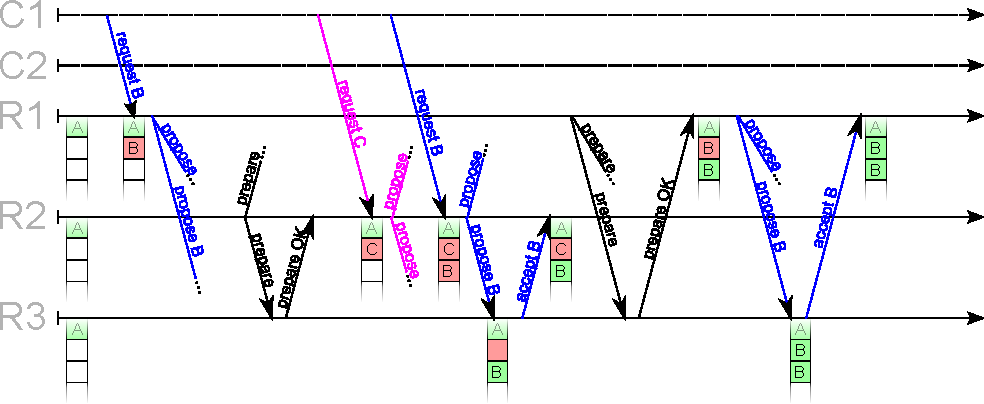
\includegraphics[keepaspectratio, width=\textwidth]{paxos/duplicating_messages.pdf}
  \caption{Duplicating messages -- the example scenario}
\end{figure}
\begin{description}
  \item[Scenario] There are three replicas - $R_1$, $R_2$ and $R_3$. $R_1$ is the leader, proposes <1:B> (value B in first consensus instance). No other processes receives these messages and $R_2$ becomes the leader. $R_2$ proposes <1:C> and <2:B>. All proposes for <1:C> are lost, but <2:B> is decided. $R_2$ fails and $R_1$ becomes the leader again. While preparing, it learns about <2:B>. It has <1:B> as a previously accepted value. The Paxos algorithm requires $R_1$ to propose <1:B> again, since its the accepted value with the highest timestamp. And this will result in the request being decided twice.
\end{description}

Unfortunately we cannot prevent requests from being decided twice in two different instances. Because of that, the only valid solution for this problem is to remember the last executed instance for every client and not executing it again. But this requires to keep a new structure in memory as well as by every snapshot (after recovering from the snapshot, this structure has to be loaded too).

Even if we cannot prevent from deciding a request twice, we should minimise the number of such situations because they slow down the algorithm (we have to send redundant data in each message). Possible solutions to decrease the scale of this problem are listed below:
\begin{itemize}
  \item We can cache the last reply for each client, so after receiving the same request we can immediately response.
  \item Do not propose requests which have been already decided
  \item The current leader can save which requests were proposed by him (but not decided yet) and also discard them.
\end{itemize}

\paragraph{Setting the window size}
The windows size specifies how many concurrent instances can be started (it has very similar meaning to the window size in the TCP protocol). In order to use available resources and keep high responsiveness the window size must be set correctly. There is no global, generic solution: every usage needs different setting.

The most important thing is monitoring the network: its usage should be high, but no congestion should occur.
That means, on one side, the window size must be enlarged as long as the links are not full, and on the other side, it must be guaranteed that no message will be delayed or dropped because of the network traffic. As long as the two conditions hold, a speed of a single instance remains constant (putting aside CPU time).
If network is overused, the overall throughput may even stay on the same level, but the latency will increase for sure.

If the instances would be decided out of order the JPaxos performance would not be affected much. But the state machine must get the requests in proper order, so the execution of requests with greater IDs would have to be delayed. And this causes inefficient request arrival time for the service. So the number of concurrent instances should not be increased if it does not increase the JPaxos throughput.

\paragraph{Performance gains}
A single instance will nearly never use available bandwidth, so conducting concurrent instances will surely speed up JPaxos.

As already mentioned, using the concurrent instances will improve latency and throughput. Carefulness is required in order to avoid network saturation, especially the link of the leader which has to carry $2n$ messages for each instance (as opposed to 2 messages for every other link).

In full-duplex networks, concurrent instances will improve network utilisation, because when the leader is waiting for replies, the network from the leader to the others is idle, so it can be used to send the next request. 

% TODO remove this paragraph?
\paragraph{Batching} is another method for improving performance and network usage. It is preferred over increasing the concurrent instances count, however joining these two methods is better than any of them alone. Batching is described in section \ref{sec:batching}, as it does not concern the Paxos protocol, but values passed to the Proposer.

\section{Batching}
\label{sec:batching}
Batching means using the same consensus instance to order several requests.

This optimisation does not need any changes to the Paxos algorithm, only requires that requests from one instance can be ordered deterministically by each replica, so that replicas know the order in which they should execute the requests. That is no problem, as a byte stream is already ordered -- so each replica will decode the requests the same way.

To achieve multiple requests in the same instance an additional activity must be taken up by the proposer and later, by replica, just before execution.

The proposer needs to \textit{stick} together the requests, and from that moment on they are treated as one. The other part, dividing it again into requests, should be done after the decision has been taken.
\begin{figure}[h]
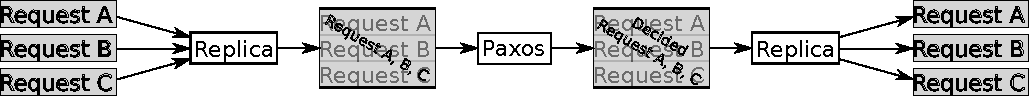
\includegraphics[keepaspectratio, width=\textwidth]{features/batching.pdf}
\vspace{-1em}
\caption{The batching mechanism}
\vspace{-1em}
\end{figure}

As the count of concurrent instances is bounded (see subsection \ref{subsec:concurrent_instances}), without batching every client needs to wait for his own instance. With batching many client requests may be \textit{packed} in one instance. That, on one side, increases the throughput and decreases the delay.
On the other side, the message size is getting bigger -- and that means slower voting.

Here arises a question: how many requests to batch? One boundary is quite obvious -- a serialized message should not be bigger than the transport protocol frame size. As for UDP the size is about 65kB, but for TCP stays unbounded.

The network bandwidth is the upper bound of peformance. Increasing the size of the instance value does not change the CPU time needed to decide on this instance. So the best performance is achieved as the batching size is set to the minimal size when all available bandwidth is used.

Another problem concerns the proposer: should there be a lower limit of requests in one instance? Doing so implies waiting for new client requests to come. Not waiting means sometimes severe throughput loss.

A new request may come a long time after we begun gathering the requests for batching -- and that would cause an unacceptable delay. So if we choose to wait for new client requests, we need to set up a timeout after which we stop waiting for the new requests and start deciding the requests we manged to gather.

If we decide not to wait at all we are packing all client requests we got until now into a single request (if it fits, of course). Such approach guarantees good behaviour if the system state is not changing. Under load  we are usually unable to pack all requests we got into single instace, while with small amount of requests no delay by packing decreases the latency.

Both the batching size and the timeout for gathering requests in a batch is configurable in our library.


\section{No operation command}

When concurrent instances optimisation is used, it is possible that leader after prepare phase will have a gap in the log. To illustrate the problem, let's analyze the scenario below.

\begin{description}
  \item [Scenario] We have three replicas $R1$, $R2$ and $R3$. Replica $R1$ is the leader and proposes <1:A> and <2:B>. Value <2:B> is decided by all replicas, but no other process receives <1:A>. $R1$ crashes and $R2$ becomes a new leader. After prepare phase, $R2$ has a gap in the log because no information about instance 1 was received.
\end{description} 

As we can see after the prepare phase, a leader can have a gap in the log. Without filling this gap, replica cannot execute and propose new values. Because of that, a new value has to be proposed in this place.

With crash-stop or crash-recovery without stable storage the value may be lost forever. That happens when decision $k+1$ is already decided, and decision $k$ is unknown to all but the leader, and the leader crashes. As only he got the value, and it has been lost -- either because he is not allowed to recover, or he is recovering without stable storage.

On the other hand, the leader change may happen due to the lost of \alive message. In this case someone has the value, and it could be used back in the voting. But there is no simple and fast method to detect this situation.

The easiest solution is to create a new request type called no-op, which is a null operation that will be ignored by the replicas. It fills the gaps but is not executed by the state machine.

\section{Log truncation}

The replicated log cannot be allowed to grow forever, it must be bounded in any practical system. After any replica executes some command, it no longer needs the corresponding log entry locally. But other replicas may not have learnt the decision yet. In this case, these late replicas need to learn the decision by asking the corresponding log entry from a replica that still has it.

In JPaxos the Paxos protocol is not used for getting lost requests due to performance reasons. For this we use a special procedure called \textit{catch-up}, which is described in section \ref{sec:catch_up}.

Having the old log is needed in three cases: for the catch-up, for view change and, in the crash-recovery model, for recovery.
The catch-up needs old log in order to send them to a replica which is not up to date, once the replica requests them.
During the view change the leader requests log entries of all instances it considers to be undecided.
By recovery a replica needs the log of other replicas in order to know what has been decided at least since its crash.

Especially the latter is problematic. The view change always requires a bounded number of instances in the log. But if we assume recovery with minimal or no stable storage (as in the case of the epoch based or view based recovery algorithm), after the recovery a replica needs to recover the state from scratch. For this, it needs the whole log or complete state.

\paragraphNewline{Global Commit Point}

A command can be deleted from the log after being executed by all replicas in crash-stop and crash-recovery models with stable storage. The highest instance executed by all replicas is called a \emph{global commit point}.

But removing all instances prior to the global commit point is not enough to ensure that the log is kept bounded, because a correct replica may be disconnected from the system for some time. When communication is reestablished, the replica needs to learn about all the decisions taken in the meantime. If one replica crashes, the other replicas have no way of knowing that it is a crash and not a disconnection, so they would have to keep the logs forever. And the replica can stay crashed for arbitrary long time.

Therefore using snapshotting is the only acceptable solution in JPaxos.

\paragraphNewline{Snapshotting}

A replica needs the old log entries in order to bring its state up to date. But instead of executing all decided requests the replica may transfer the state of the service from other replica. To transfer the state of the service some assumption must be fullfilled: the service must be able to save its state, and be able to update itself to such state.

The service can create a \textit{snapshot} -- arbitrary data that can be parsed by the service to change its state to the state identical as in the moment when the snapshot was created.

The mechanism of managing such snapshots is called by us \textit{snapshotting}.

In order to be able to remove stale log entries snapshotting must to be implemented. It also speeds up the recovery and process of filling missing instances.

The size of a snapshot is of course bounded. If we create a new snapshot as the log size reaches some limit the size of the log is bounded as well, so no structure is allowed to grow forever.

When a new snapshot is created the old log entries are truncated. If a replica that is missing old logs rejoins, the most recent snapshot is transferred first and then all the decisions since the snapshot are sent to complete the updating procedure.

The most problematic part is the Service -- if it does not implement creating snapshots or does not provide them often enough, the log will grow forever.

Snapshotting is described in details in the section \ref{sec:snapshotting}.

\section{Skipping redundant messages}
Reducing the number of messages is one of the most efficient optimisations. In JPaxos a process does not send messages to itself, also the proposer does not send \accept messages to anyone.

It has been proven for the Paxos consensus algorithm that it minimises the number of messages carrying a value to be agreed upon (the client request in our case). The value is sent only once to each replica (not counting retransmission due to message loss). As for additional messages, their count varies among certain implementations. Some of messages proposed in the typical implementation may be easily skipped without violating guarantees or adding any assumptions.

\paragraphNewline{Using {\normalfont\propose}as {\normalfont\accept}}

Another optimisation is merging the role of \accept and \textsc{Propose}. As long as acceptors and proposes do not share the log this is not allowed. But if their knowledge is identical and the leader proposed some value, then he must accept it as well. In most solutions one node acts as proposer and acceptor, and they do share the log.

So in JPaxos each \propose is simultaneously an \accept message. Notice that if the system consists of three nodes every process decides on the value by receiving a valid propose -- it knows that the leader and itself
accept the message. Normally the leader process has to first send \propose to all and later \accept to all. By this optimisation only half of messages is required to be sent.

\paragraphNewline{Sending to itself}

As stated before, Paxos defines three types of roles: proposers, acceptors and learners. Processes or some of their parts act as one of them. In order to communicate they must send messages to each other.

In our program every node consists of a (probable) proposer, acceptor as well as learner. In this case there is no need to send messages to self. Especially all send-to-all commands may be replaced by send to others command, as long as the communication with self will be done internally. This skips one \accept and one \propose sent by the leader, and one \accept by all other processes.

This does not influence performance much, however it is recommended as it decreases the use of system resources (especially the networking stack). It also skips a few system calls.

\paragraphNewline{Minimizing the count of messages carrying the value}

Most of the articles about Paxos state that the \accept message carries the value (request from client).
In such case we can accept on the value even without receiving a \propose message.

The value usually is bigger than a normal message of JPaxos. Because of that we want to minimize number of messages which contain the value.
In JPaxos the \accept message does not carry the value. Before a process can send the \accept message it has to receive the \propose message. The process decides upon a value if it receives a \propose and majority of \accept messages.

Waiting for the \propose message might cause additional overhead, but usually the \propose will be delivered prior to the majority of \accept messages.
Each process must receive one \propose[], but multiple \accept messages. If the \accept message does not carry the value, significantly less network bandwidth is used by a single instance.


\paragraphNewline{Best-case messages}
\label{par:bestCaseMessages}
So, in the normal operation in JPaxos:

%TODO: TZ: Jeśli masz sprawnego inkscape'a, narysuj proszę do tego prosty rysunek best case 
% mi nie tylko vim'a popsuł niedokończony update systemu, inkscape też narzeka na brak jakiegoś .so
% chodzi o diagram odpowiadający komunikacjom z tabelki poniżej

\begin{table}[h]
\begin{tabular}{rccccc}
          & \begin{tabular}{c} How many \\ processes send \\ the message \end{tabular} 
          & \begin{tabular}{c} Count of \\ messages \\ sent \end{tabular} 
          & Time 
          & \begin{tabular}{c} Message \\ type \end{tabular}
          & \begin{tabular}{c} Carries value \\ (client requests) \end{tabular}
          \\
 Proposer & $1$                     & $n-1$             & $n$  & \propose & yes    \\
 Acceptor & $n-1$                   & $n-1$             & 1    & \accept  & no
\end{tabular}
\end{table}

We can see that in order to decide the process needs to send the \propose[] once, and later each non-leader process sends the \accept to others.

For the comparison of consensus algorithms usually time is defined in a specific way: $n$ denotes the time needed to send a message containing the value to be agreed upon, and $1$ is the time required to send any other message. This is motivated by the value size -- usually the value is significantly bigger than any protocol message, so it is important to differentiate the messages carrying value and all the others.

Other implementations consider using bounded learner count -- only some processes are selected as the learners. For example only one process plays the role of a learner -- that means the acceptors send the \accept messages only to this process. An additional message, \textsc{Decided}, is sent by the learner to all as the ballot has finished. Thanks to this modification no reliable broadcast is needed, but also an additional phase of communication must occur. If only some processes act as learners, it is important to ensure that there is at least one learner that didn't crash, otherwise the protocol would not guarantee liveness.

An interesting approach is presented in the RingPaxos (see \cite{Mar10}), where IP-multicast is used for all broadcasts, what significantly increases the scalability and performance.
